\subsection{Evaluating Performance Comparison Results}

\textbf{Did you learn what you wanted from the programs and experiments?}

\textbf{How did the program performance compare to its selected standard?} 
Evaluate the performance criteria against the other published results. 

\textbf{Did the program demonstrate good performance?}
All results gave better results than plain ACO implementation.
Number of direct transfers: competitive with other approaches. Average travel time: better. 

\textbf{Is the programs performance different from predictions?} When it comes to comparing the proposed algorithm with the plain ACO implementation: We did expect the program to be better. ACO has, as mentioned, a known limitation of getting stuck at a local optima. This is very well demonstrated in Figure \ref{fig:acovssso}, which shows the average growth in the $TOTFIT$ value for each iteration of ACO and SSO. (10 runs for each algorithm is run. For each iteration, the average $TOTFIT$ value among each run is recorded.) As one can observe, the ACO implementation manage to find good solutions fast, by following pheromone trails laid by previous ants. But after around 35 iterations, the algorithm is unable to find better solutions. The amount of pheromone on the first best paths only increase, and unable ants to explore possible better routes. As one can see, the proposed SSO algorithm manage to get out of this inconvenience. Notion of global best solution, crazy ants, following ants reward best edges, memory etc.


%\citet{poorzahedy11} reports that ``In more than 80\% of the time, the best found solution of the problem has been found in less than 65 iterations'' --> Settes i sammenheng med $i$.

 \begin{figure}[H]
    \begin{center}
    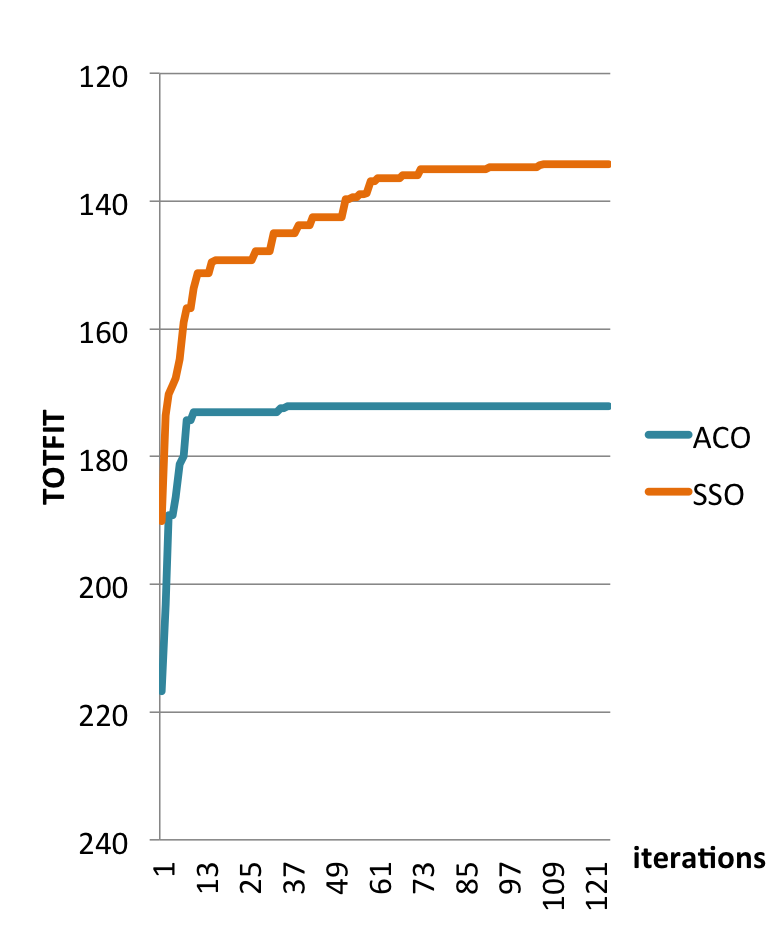
\includegraphics[width=3in]{assets/acovsssoNEW.png}
    \end{center}
    \caption{Evolution of TOTFIT for ACO and SSO }
    \label{fig:acovssso} 
\end{figure}

As one can observe in \vref{table:performanceComparison_routesets}, the amount of direct travelers increase with in line with the number of route sets. This makes sense because thus more route sets the passenger can choose from, thus bigger probability for the passenger to find a route that is convenient for him / her. This is well demonstrated when comparing the graphs of four route sets, \vref{fig:bestRouteSet4}, and six route sets, Figure \vref{fig:bestRouteSet6}.  

 \begin{table}[H]
    \centering
    \begin{tabular}{|l||l|l|l|l|l|}
    \hline
    Route Set & $d_0(\%)$ & $d_1(\%)$ & $d_2(\%)$ & $d_{unsat}(\%)$ & $ATT$ \\
    \hline
    4 & 85.21 & 13.49 & 1.30 & 0.00 & 10.27\\
    \hline
    6 & 87.17 & 12.0 & 0.82 & 0.01 & 10.11\\
    \hline
    7 \\
    \hline
    \end{tabular}
    \caption {Evaluating increase of Route Sets}
    % 50 runs
    \label{table:performanceComparison_routesets}
\end{table}